\documentclass{amsart}
\usepackage{amsmath}
\usepackage{amssymb}
\usepackage{amsthm}
\usepackage{enumerate}
\usepackage{hyperref}
\usepackage{graphicx} 
\author{Alex Thies}
\title{Homework 0 \\ Math 463 - Spring 2017}
%\email{athies@uoregon.edu}
\begin{document}
	\maketitle
	
	\section{Assignment} % (fold)
	\label{sec:assignment}
	The purpose of this short assignment is to learn how to load an external data file into R, perform elementary operations on a data frame, and fit a simple linear regression model.
	The data for this lab can be found at \url{http://www.uoregon.edu/~dlevin/DATA/mus.txt}.
	The variables are LOCATION, AGE, and WEIGHT. The data gives the weight and age of mussels collected at two locations.
	Plot the relationship between weight and age for all the data. Use a different symbol for the two locations.
	Fit a linear regression model for each location separately, and plot the regression lines on the same graph as above.
	Report the estimated parameters and their standard errors.	
	% section assignment (end)
	
	\section{Report} % (fold)
	\label{sec:report}
		\subsection{Introduction} % (fold)
		\label{sub:introduction}
			I collaborated with Ashley Ordway on this assignment.
		% subsection introduction (end)
		\subsection{Findings} % (fold)
		\label{sub:findings}
			As instructed, we make the following plot, and associated least-squared lines.
			\begin{figure}[h]
				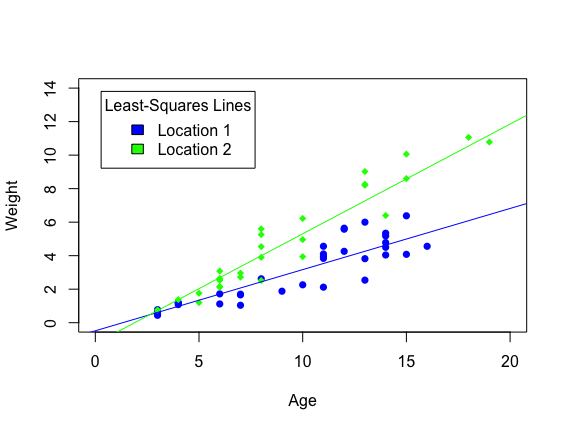
\includegraphics[width=0.7\linewidth]{musplot.png}
				\caption{Weight as Age}
				\label{fig1}
			\end{figure}

			Furthermore, we report the estimated coefficients of the respective least-squared lines, and their standard error.

			\begin{figure}
				\begin{tabular}{c|ccc}
					\hline
					Location & $\hat{\beta_{0}}$ & $\hat{\beta_{1}}$ & SE \\
					\hline \\
					1 & -0.4828 & 0.3649 & 0.35542 \\
					\hline \\
					2 & -1.2420 & 0.6549 & 0.03114 \\
					\hline
				\end{tabular}
				\caption{Least-square line parameters}
				\label{fig2}
			\end{figure}

		% subsection findings (end)
	% section report (end)
\end{document}